% !TEX root = ../../seminar.tex

\subsection{Evaluate Process}
\label{subsec:evaluate process}

The last step is to reflect on the whole process. After discussing the study, Dyb{\aa} \etal recommend to reflect on how well each step was performed and to find improvements for the next iteration. To support this they recommend using \emph{after-action reviews} (AAR) and \emph{postmortem analysis} (PMA) \cite{Dyba2005}.

AAR is a short meeting of 10 to 20 minutes to answer the four questions in figure \ref{fig:aar_pma}, left box. This method can also be used at any other point during the process if there is a need for reflection or rethinking the current situation \cite{Dyba2005}.

PMA is similar to AAR but with a deeper insight. Therefore it lasts for several hours up to a full day. It answers the questions in figure \ref{fig:aar_pma}, right box \cite{Dyba2005}. Here, conclusions can be drawn to improve upcoming EBSE cycles and further research in general. This method can give insight in issues. For example:
\begin{itemize}
\item Which methods worked out as planned and which did not?
\item Where was time lost and deadlines missed?
\item Which technique proves to be used in upcoming studies?
\end{itemize}

After this step the current iteration of the process is finished. It can be started over again with the next research question.

\begin{figure}
	\centering
	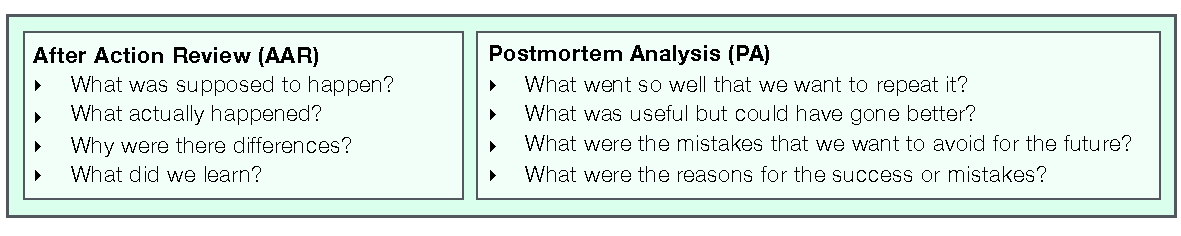
\includegraphics[width=12.5cm]{figures/aar_pma.pdf}
	\caption{After-action reviews (AAR) left box, and postmortem analysis (PMA) right box \cite{Dyba2005}.}
	\label{fig:aar_pma}
\end{figure}
